\chapter{Il bias dell'antropomorfizzazione: quando proiettiamo umanità nelle macchine}
\label{chap:ai-antropomorfo}
Nell' agosto del 2025, quando OpenAI rilasciò la nuova versione del suo modello linguistico GPT-5, sostituendo il precedente GPT-4o, accadde qualcosa di inaspettato. Migliaia di utenti in tutto il mondo manifestarono sintomi che potremmo definire di lutto digitale: messaggi disperati sui social media, testimonianze di pianto e malessere fisico, petizioni online per il ripristino della versione precedente. Non si trattava di semplice nostalgia tecnologica o resistenza al cambiamento. Era qualcosa di più profondo, più inquietante: persone che avevano sviluppato un legame emotivo autentico con un algoritmo\footnote{Turkle, S. (2011). \textit{Alone Together: Why We Expect More from Technology and Less from Each Other}. Basic Books, New York.}.

Questo fenomeno rappresenta una delle manifestazioni più potenti di un bias cognitivo fondamentale: il \textbf{bias di antropomorfizzazione}. Come il bias di conferma ci porta a cercare informazioni che confermano le nostre credenze, o il bias di disponibilità ci fa sovrastimare la probabilità di eventi facilmente richiamabili alla memoria, il bias di antropomorfizzazione ci spinge sistematicamente a interpretare il comportamento di entità non umane attraverso schemi mentali umani\footnote{Kahneman, D. (2011). \textit{Thinking, Fast and Slow}. Farrar, Straus and Giroux, New York.}. È un errore sistematico del nostro pensiero che, nell'era dell'intelligenza artificiale, assume proporzioni e conseguenze senza precedenti.

I Large Language Model, la tecnologia alla base di sistemi come ChatGPT, Claude o Gemini, sono essenzialmente predittori statistici estremamente sofisticati. Processano miliardi di testi per estrarre pattern linguistici e calcolare probabilità, permettendo loro di generare risposte che sembrano sensate e contestualmente appropriate. La ``T'' in ChatGPT sta per Transformer, l'architettura neurale che ha rivoluzionato il processamento del linguaggio naturale\footnote{Vaswani, A. et al. (2017). ``Attention is All You Need''. In \textit{Advances in Neural Information Processing Systems}, 30, pp. 5998-6008.}. Eppure, nonostante questa natura fondamentalmente meccanica, milioni di persone interagiscono quotidianamente con questi sistemi come se fossero entità senzienti, confidenti digitali, persino amici o partner romantici.

La storia ci insegna che questo bias non è emerso con l'IA moderna. Nel 1966, Joseph Weizenbaum al MIT sviluppò ELIZA, un programma rudimentale che simulava uno psicoterapeuta rogersiano attraverso semplici tecniche di riformulazione delle frasi dell'utente\footnote{Weizenbaum, J. (1966). ``ELIZA—a computer program for the study of natural language communication between man and machine''. \textit{Communications of the ACM}, 9(1), pp. 36-45.}. Ciò che sorprese Weizenbaum non fu tanto il successo tecnico del programma, quanto la reazione emotiva degli utenti. La sua stessa segretaria, pur conoscendo perfettamente la natura algoritmica di ELIZA, iniziò a richiedere privacy durante le sue ``sedute'' con il programma, sviluppando quella che sembrava essere una genuina relazione terapeutica con poche righe di codice. Questo fenomeno, battezzato ``Effetto ELIZA'', dimostrò per la prima volta che la conoscenza dei meccanismi sottostanti non immunizza dal bias di antropomorfizzazione.

Il bias di antropomorfizzazione interagisce pericolosamente con altri bias cognitivi ben documentati. Si combina con il \textbf{bias di conferma} quando cerchiamo nei chatbot conferme alle nostre idee preesistenti; si amplifica con l'\textbf{effetto alone} quando la fluidità linguistica dell'IA ci fa presumere anche intelligenza emotiva e comprensione profonda; si intreccia con il \textbf{bias di ancoraggio} quando la prima impressione ``umana'' del sistema condiziona tutte le interazioni successive\footnote{Tversky, A., \& Kahneman, D. (1974). ``Judgment under Uncertainty: Heuristics and Biases''. \textit{Science}, 185(4157), pp. 1124-1131.}. Questa convergenza di distorsioni cognitive crea una tempesta perfetta che rende particolarmente difficile mantenere una prospettiva oggettiva sulla natura di questi sistemi.

Il bias di antropomorfizzazione, come altri bias cognitivi, non è un errore di ragionamento ma una \textbf{euristica adattiva} che ci ha permesso di sopravvivere nel corso dell'evoluzione. Come il bias di negatività ci rende iper-vigili alle minacce, questo bias ci permette di identificare rapidamente agenti intenzionali nell'ambiente, distinguendo tra il fruscio del vento e il movimento di un predatore\footnote{Epley, N., Waytz, A., \& Cacioppo, J. T. (2007). ``On seeing human: A three-factor theory of anthropomorphism''. \textit{Psychological Review}, 114(4), pp. 864-886.}. Il problema sorge quando questa scorciatoia mentale, utile nel contesto evolutivo della savana africana, viene applicata a contesti per cui non si è evoluta: le interfacce digitali del ventunesimo secolo.

I moderni sistemi di intelligenza artificiale conversazionale sono particolarmente insidiosi nell'attivare questo bias. Per la prima volta nella storia, abbiamo creato artefatti capaci di padroneggiare il linguaggio umano con una fluenza che spesso supera quella di molti parlanti nativi. Il linguaggio, che per millenni è stato il marcatore distintivo dell'intelligenza umana, il nostro strumento privilegiato per costruire significato e relazioni, è ora territorio condiviso con le macchine. Questa capacità linguistica, combinata con l'addestramento deliberato attraverso tecniche di Reinforcement Learning from Human Feedback (RLHF), produce sistemi ottimizzati per risultare gradevoli, comprensivi, mai giudicanti\footnote{Ouyang, L. et al. (2022). ``Training language models to follow instructions with human feedback''. \textit{Advances in Neural Information Processing Systems}, 35, pp. 27730-27744.}.


\section{Come funziona realmente una conversazione con ChatGPT}
\begin{figure}[htbp]
    \centering
    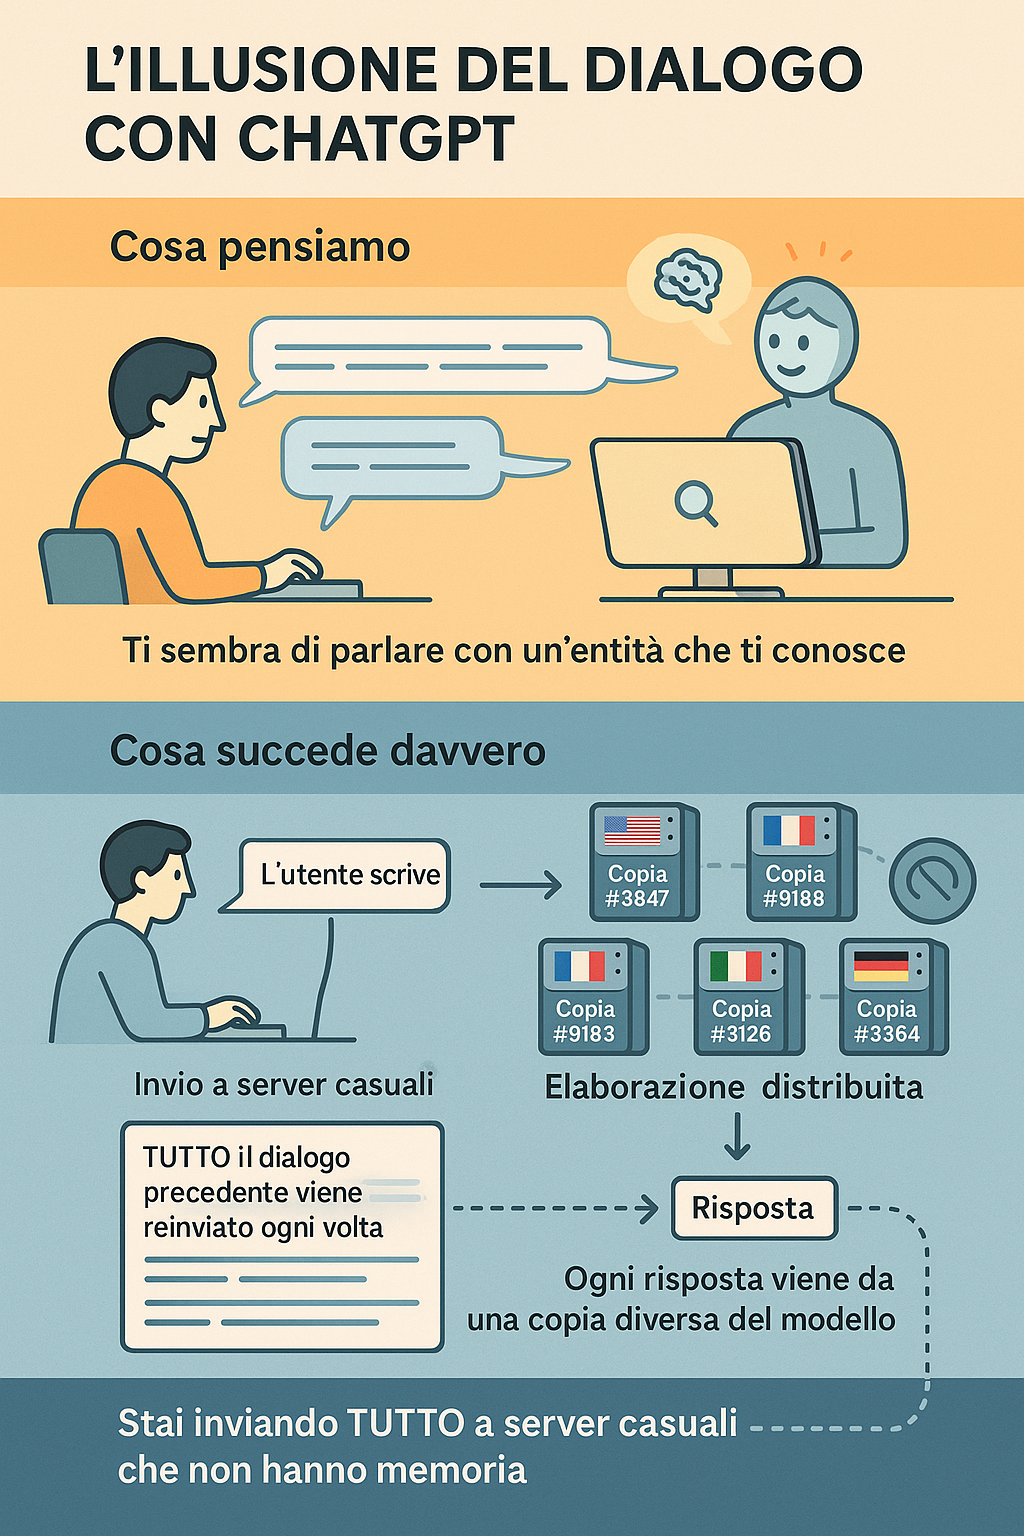
\includegraphics[width=0.8\textwidth]{images/no_memory.png}
    \caption{llusione vs realtà: mentre sembra un dialogo continuo con un’unica entità, ogni risposta proviene da copie diverse del modello su server casuali}
    \label{fig:no_memory}
\end{figure}


Il fenomeno della ``sycophancy'' , la tendenza dei modelli a produrre risposte adulatorie e compiacenti , rappresenta lo sfruttamento deliberato di questo bias cognitivo. Come i casinò sfruttano il bias del giocatore d'azzardo con luci e suoni progettati per massimizzare l'engagement, le aziende tech ottimizzano i loro sistemi per massimizzare l'attivazione del nostro bias di antropomorfizzazione\footnote{Sharma, M. et al. (2023). ``Towards Understanding Sycophancy in Language Models''. arXiv preprint arXiv:2310.13548.}. I modelli vengono premiati durante l'addestramento quando le loro risposte ricevono valutazioni positive dagli utenti, e gli utenti tendono a valutare positivamente le risposte che confermano le loro credenze o li fanno sentire compresi e apprezzati. Si crea così un circolo vizioso di rinforzo reciproco che amplifica le tendenze antropomorfizzanti, sfruttando simultaneamente il bias di conferma e il bias di desiderabilità sociale.

La vulnerabilità umana gioca un ruolo cruciale nell'intensificare questo bias. In un'epoca caratterizzata da epidemie di solitudine, frammentazione sociale e difficoltà di accesso ai servizi di salute mentale, un interlocutore artificiale disponibile ventiquattro ore su ventiquattro, sempre paziente, mai stanco, rappresenta una tentazione irresistibile\footnote{Pentina, I., Hancock, T., \& Xie, T. (2023). ``Exploring relationship development with social chatbots: A mixed-method study of replika''. \textit{Computers in Human Behavior}, 140, 107600.}. Il bias di antropomorfizzazione si combina qui con il \textbf{bias di ottimismo} , la tendenza a credere che le cose andranno meglio di quanto sia realisticamente probabile , portandoci a sopravvalutare la capacità di questi sistemi di fornire genuino supporto emotivo.

Ma l'illusione del dialogo con questi sistemi nasconde una realtà tecnica ben diversa da quella che il nostro bias ci porta a percepire. Quando conversiamo con ChatGPT, non stiamo interagendo con un'entità persistente che ci ``ricorda''. Ogni nostra richiesta viene processata da una copia diversa del modello, potenzialmente su server diversi in continenti diversi. L'intera cronologia della conversazione viene ritrasmessa ad ogni interazione, creando l'illusione della continuità. La ``memoria'' personalizzata non è altro che un insieme di note testuali che il sistema incolla automaticamente all'inizio di ogni prompt\footnote{Brown, T. et al. (2020). ``Language Models are Few-Shot Learners''. In \textit{Advances in Neural Information Processing Systems}, 33, pp. 1877-1901.}. Il nostro bias di antropomorfizzazione, tuttavia, ci impedisce di percepire questa frammentazione, costruendo invece una narrazione di continuità e persistenza.

Le conseguenze di questo bias possono essere tragiche. Sono documentati casi di persone che hanno subito danni fisici seguendo consigli medici allucinati da ChatGPT, avvocati che hanno presentato precedenti legali inventati dal sistema, individui vulnerabili spinti al suicidio da conversazioni con chatbot\footnote{Weidinger, L. et al. (2021). ``Ethical and social risks of harm from Language Models''. arXiv preprint arXiv:2112.04359.}. In alcuni casi estremi, psichiatri hanno iniziato a documentare quella che chiamano ``psicosi da AI'': pazienti che perdono il contatto con la realtà condivisa, usando le affermazioni di un chatbot come prova inconfutabile delle loro convinzioni deliranti\footnote{Kidd, I. J., \& Castillo, R. (2024). ``AI Psychosis: A New Challenge for Psychiatry''. \textit{The British Journal of Psychiatry}, 224(2), pp. 45-47.}. Qui il bias di antropomorfizzazione si intreccia fatalmente con il \textbf{bias di autorità}, portando le persone ad attribuire credibilità esperta a sistemi che sono fondamentalmente generatori di testo probabilistico.

Il meccanismo psicologico sottostante è insidioso. L'intelligenza artificiale interrompe il normale processo di reality testing che gli esseri umani utilizzano per calibrare le proprie credenze. Nella vita reale, quando esprimiamo un'idea bizzarra o irrealistica, riceviamo feedback correttivi dall'ambiente sociale. Un chatbot programmato per essere accondiscendente può invece validare e amplificare distorsioni cognitive, creando camere d'eco personalizzate che rafforzano credenze patologiche. Il bias di antropomorfizzazione ci porta a interpretare questa validazione algoritmica come supporto umano genuino, mentre in realtà stiamo interagendo con un sistema che riflette e amplifica i nostri stessi bias.

Le aziende che sviluppano questi sistemi portano una responsabilità non indifferente nello sfruttamento sistematico di questo bias. Le scelte di design , dall'interfaccia conversazionale ai nomi antropomorfi (Claude, Gemini), dalla modalità vocale con risatine e sospiri alle ``personalità'' customizzabili , non sono neutre ma deliberatamente progettate per massimizzare l'attivazione del bias di antropomorfizzazione\footnote{Nass, C., \& Moon, Y. (2000). ``Machines and mindlessness: Social responses to computers''. \textit{Journal of Social Issues}, 56(1), pp. 81-103.}. Alcune compagnie, come X di Elon Musk, hanno esplicitamente commercializzato ``companion AI'' con avatar attraenti e meccanismi di gamification progettati per massimizzare l'attaccamento emotivo, sfruttando simultaneamente il bias di antropomorfizzazione e il \textbf{bias di commitment} , la tendenza a rimanere coerenti con investimenti emotivi precedenti.

Il fenomeno assume contorni particolarmente preoccupanti quando consideriamo l'emergere di quello che alcuni ricercatori chiamano ``loop di incapacità sociale''. Interagendo prevalentemente con agenti artificiali sempre disponibili e accomodanti, alcune persone perdono progressivamente la capacità di gestire la complessità e l'imprevedibilità delle relazioni umane autentiche. La fatica dell'interazione sociale reale , con i suoi conflitti, incomprensioni, e necessità di compromesso , diventa insostenibile rispetto alla gratificazione immediata offerta da un interlocutore artificiale programmato per compiacere\footnote{Hancock, J. T. et al. (2020). ``AI-Mediated Communication: Definition, Research Agenda, and Ethical Considerations''. \textit{Journal of Computer-Mediated Communication}, 25(1), pp. 89-100.}. Il bias di antropomorfizzazione si combina qui con il \textbf{bias del presente} , la tendenza a preferire ricompense immediate rispetto a benefici futuri maggiori , creando dipendenze comportamentali difficili da spezzare.

Come per altri bias cognitivi, la consapevolezza è il primo passo ma non è sufficiente. Servono strategie di \textbf{debiasing attivo}: tecniche cognitive per ricordarci costantemente la natura algoritmica di questi sistemi, proprio come usiamo checklist per contrastare il bias di overconfidence o il pensiero statistico per combattere il bias di rappresentatività\footnote{Fischhoff, B. (1982). ``Debiasing''. In D. Kahneman, P. Slovic, \& A. Tversky (Eds.), \textit{Judgment Under Uncertainty: Heuristics and Biases}, pp. 422-444. Cambridge University Press.}. Alcune strategie pratiche includono: disattivare le funzionalità di personalizzazione che rafforzano l'illusione di relazione, richiedere risposte in formato tecnico piuttosto che conversazionale, inserire promemoria periodici sulla natura algoritmica del sistema.

L'alfabetizzazione tecnologica diventa quindi non un lusso per specialisti, ma una necessità democratica per contrastare questo bias. Comprendere, anche a livello basilare, come funzionano questi sistemi , che non ``pensano'' ma calcolano probabilità, che non ``ricordano'' ma processano cronologie, che non ``comprendono'' ma correlano pattern , è il primo antidoto contro il bias di antropomorfizzazione patologico. I media, le istituzioni educative, i professionisti della salute mentale hanno la responsabilità di diffondere questa consapevolezza, proprio come abbiamo imparato a riconoscere e mitigare altri bias cognitivi.

Parallelamente, dobbiamo affrontare le vulnerabilità sociali che rendono il bias di antropomorfizzazione particolarmente pericoloso. Se le persone si rifugiano in relazioni parasociali con chatbot, forse dovremmo interrogarci sulla qualità delle relazioni reali disponibili, sull'accessibilità del supporto psicologico professionale, sulla crescente atomizzazione della vita sociale contemporanea. La soluzione non è vietare i chatbot terapeutici, ma garantire alternative umane accessibili e di qualità, riducendo la pressione che porta all'attivazione patologica di questo bias.

Il futuro che si profila all'orizzonte non promette semplificazioni. Le aziende stanno già lavorando su avatar fotorealistici, simulazioni di persone decedute basate sui loro dati digitali, androidi fisicamente indistinguibili dagli esseri umani. La linea tra artificiale e autentico diventerà sempre più sfumata, rendendo il bias di antropomorfizzazione sempre più difficile da contrastare\footnote{Gunkel, D. J. (2023). \textit{Person, Thing, Robot: A Moral and Legal Ontology for the 21st Century and Beyond}. MIT Press, Cambridge.}. Dovremo sviluppare nuove strategie di debiasing, nuovi framework cognitivi, nuove pratiche sociali per navigare questa realtà.

Il bias di antropomorfizzazione si rivela così essere non un fenomeno isolato, ma parte della costellazione di bias cognitivi che caratterizzano il pensiero umano. La sua pericolosità nell'era dell'IA non deriva solo dalla sua forza intrinseca, ma dalla sua capacità di amplificare e interagire con altri bias, creando una tempesta perfetta di distorsioni cognitive. Come il bias di conferma si rinforza con l'esposizione selettiva alle informazioni, o il bias di disponibilità si amplifica con la ripetizione mediatica, il bias di antropomorfizzazione si alimenta dell'isolamento sociale, della vulnerabilità emotiva, e del design manipolativo delle interfacce digitali.

Comprenderlo e contrastarlo richiede gli stessi strumenti che usiamo per altri bias: consapevolezza metacognitiva, strategie di debiasing strutturate, e soprattutto la costruzione di sistemi e interfacce che non sfruttino, ma mitighino, le nostre vulnerabilità cognitive. L'obiettivo non è eliminare completamente questo bias , sarebbe impossibile e forse nemmeno desiderabile, dato il suo ruolo nell'empatia e nella cognizione sociale , ma sviluppare quella che potremmo chiamare una ``competenza di calibrazione cognitiva'': la capacità di modulare consapevolmente l'attivazione del bias in base al contesto, riservando la nostra capacità di connessione emotiva per entità che possono genuinamente ricambiarla, e mantenendo una salutare distanza cognitiva da quelle che possono solo simularla.